\begin{pastexam}[label={px:ntu-114-bmei-ca-02}]{臺大生醫電資所 114 學年度 第 2 題}
（問答）

(8\%) Please draw the binary tree for the expression ``(A*(E/(B-F)))*(A+B)/D'' and write prefix and postfix forms.
\end{pastexam}

\begin{pastsoln}
\texttt{*} 和 \texttt{/} 優先順序相同、由左往右結合，所以最外層是
\[
\big((A * (E / (B - F))) * (A + B)\big) / D,
\]
最後做的是 \texttt{/}，它是樹根。 運算式樹：內部節點是運算子，左右子樹是它的兩個運算元，葉子是變數
（資結書第~7.7~節）。 由外往內拆：
\begin{itemize}
\item 根 \texttt{/}：左邊 $(A * (E/(B-F))) * (A + B)$，右邊 $D$。
\item 左子 \texttt{*}：左邊 $A * (E/(B-F))$，右邊 $A + B$。
\item $A * (E/(B-F))$：根 \texttt{*}，左 $A$，右 \texttt{/}（左 $E$，右 \texttt{-}（左 $B$，右 $F$））。
\end{itemize}
\begin{center}
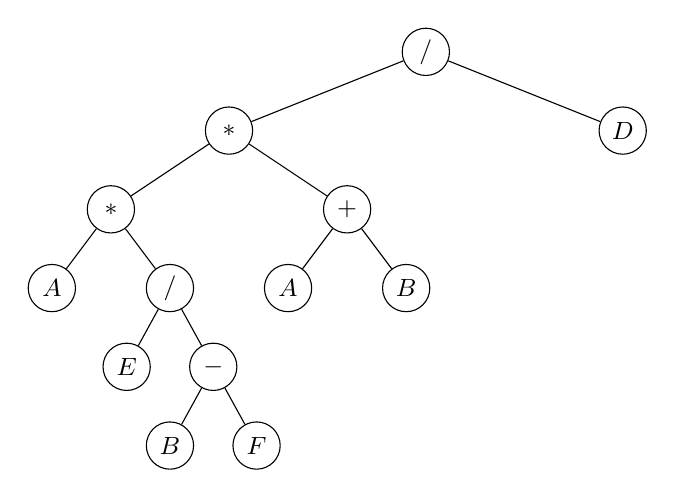
\begin{tikzpicture}[every node/.style={circle,draw,inner sep=1pt,minimum size=6mm,font=\small},level distance=10mm,edge from parent/.style={draw},level 1/.style={sibling distance=50mm},level 2/.style={sibling distance=30mm},level 3/.style={sibling distance=15mm},level 4/.style={sibling distance=11mm}]
\node {/}
  child {node {$*$}
    child {node {$*$}
      child {node {$A$}}
      child {node {/} child {node {$E$}} child {node {$-$} child {node {$B$}} child {node {$F$}}}}}
    child {node {$+$} child {node {$A$}} child {node {$B$}}}}
  child {node {$D$}};
\end{tikzpicture}
\end{center}
前序走訪（根、左、右）得到前序式，後序走訪（左、右、根）得到後序式（資結書第~6.3.5~節）：
\begin{itemize}
\item prefix：\texttt{/ * * A / E - B F + A B D}
\item postfix：\texttt{A E B F - / * A B + * D /}
\end{itemize}
檢查後序式：用堆疊求值，讀到 \texttt{-} 時算 $B - F$，\texttt{/} 算 $E/(B-F)$，\texttt{*} 算 $A * \ldots$；
再算 $A + B$，\texttt{*} 把兩者相乘；最後 $D$、\texttt{/}。 和原式的計算順序一致。

若把原式讀成 $(\ldots) * \big((A + B)/D\big)$ 就錯了：同優先順序的運算子要由左往右做，先乘再除。
\end{pastsoln}
